\section{Experiments}
\label{sec:experiment}



% We now present the experimental results and analyses.
% We begin by outlining the overall setup, 
% then evaluate the score correlation to the teacher model, assess its performance on aesthetic viewpoint suggestion,
% and analyze how the learned aesthetic field supports stable gradient-based pose optimization.
% Finally, we present ablation studies to examine the impact of different design choices and components.
\subsection{Experiment Setup}
\noindent\textbf{Datasets.}
We use RealEstate10k (RE10k)~\cite{re10k} and DL3DV~\cite{dl3dv} for training and evaluation. RE10k mainly contains indoor videos, while DL3DV involves more diverse scenes. Both have camera parameters at each frame. More details can be found in the Supplementary Material.

\noindent\textbf{Implementation Details.} We implement our framework in Pytorch~\cite{paszke2019pytorch}, using DepthSplat~\cite{depthsplat} as the feedforward Gaussian Splatting backbone. We use the VEN~\cite{wei2018good} model as the teacher for distilling aesthetic representations. VEN is a CNN model, and we use features from the $23^{rd}$ layer($14\times 14\times 512$) as the distillation target. Following Xu~\etal~\cite{depthsplat}, we use image resolutions of $256\times256$ for RE10k and $256\times448$ for DL3DV. During training, we randomly sample 2 input views for RE10k and 2 to 6 input views for DL3DV, following the same protocol as Xu~\etal~\cite{depthsplat}. More implementation and training details can be found in the Supplementary Material.

% We train the framework with batch size 8, learning rate $0.0005$, AdamW~\cite{adamw} optimizer and cosine annealing scheduler for $25,000$ iterations.

\noindent\textbf{Search Pipeline Configurations.} At inference, we search for optimal views via a two-stage approach. In Stage 1, within each segment of the interpolated trajectory, we uniformly sample 16 camera poses, and around each we further sample 8 neighboring poses. We take top-2 candidates as input to the next stage. In Stage 2, we use the Adam~\cite{kingma2014adam} optimizer with step size 0.01 and update for 25 steps.
\begin{table}[t]
\small
  \centering
  \begin{subtable}[t]{0.9\linewidth}
  % \centering
  \begin{tabular}{l| c | c c c c}
    \toprule
    \multirow{2}{*}{Methods} & \multirow{2}{*}{\#Views} & \multicolumn{2}{c}{RE10k~\cite{re10k}} & \multicolumn{2}{c}{DL3DV~\cite{dl3dv}} \\
     & & PLCC & SRCC & PLCC & SRCC \\
    \midrule
    Baseline & \multirow{2}{*}{2} & 0.657 & 0.628 & 0.326 & 0.307 \\
    \textbf{Ours} & & \textbf{0.780} & \textbf{0.740} &  \textbf{0.509} & \textbf{0.477} \\
    \midrule
    Baseline & \multirow{2}{*}{4} & 0.657 & 0.633 & 0.513 & 0.481\\
    \textbf{Ours} & & \textbf{0.796} & \textbf{0.758} &  \textbf{0.722} & \textbf{0.682} \\
    \midrule
    Baseline & \multirow{2}{*}{6} & 0.745 & 0.701 & 0.580 & 0.553\\
    \textbf{Ours} & & \textbf{0.836} & \textbf{0.794} &  \textbf{0.753} & \textbf{0.719}\\
    \bottomrule
  \end{tabular}
  \caption{Image resolution $256\times 256$.}
  \label{tab:correlation256}
  \end{subtable}
  \vfill
  \begin{subtable}[t]{0.9\linewidth}
  \begin{tabular}{l| c | c c c c}
    \toprule
    \multirow{2}{*}{Methods} & \multirow{2}{*}{\#Views} & \multicolumn{2}{c}{RE10k~\cite{re10k}} & \multicolumn{2}{c}{DL3DV~\cite{dl3dv}} \\
     & & PLCC & SRCC & PLCC & SRCC \\
    \midrule
    Baseline & \multirow{2}{*}{2} & 0.634 & 0.611 & 0.299 & 0.286 \\
    \textbf{Ours} & & \textbf{0.733} & \textbf{0.704} & \textbf{0.479} & \textbf{0.445} \\
    \midrule
    Baseline & \multirow{2}{*}{4} & 0.596 & 0.578 & 0.552 & 0.535 \\
    \textbf{Ours} & & \textbf{0.753} & \textbf{0.722} & \textbf{0.700} & \textbf{0.668} \\
    \midrule
    Baseline & \multirow{2}{*}{6} & 0.711 & 0.656 & 0.646 & 0.625 \\
    \textbf{Ours} & & \textbf{0.821} & \textbf{0.764} & \textbf{0.737} & \textbf{0.707} \\
    \bottomrule
  \end{tabular}
  \caption{Image resolution $256\times 448$.}
  \label{tab:correlation448}
\end{subtable}
\caption{Novel view aesthetic score correlation between predicted and ground-truth scores.}
\label{tab:correlation}
\end{table}

\begin{figure}[t]
\centering
    \includegraphics[width=\linewidth]{figs/nva_1_vertical.pdf}
    \caption{(a) Aesthetic score predictions over consecutive frames. Our method produces scores closer to the ground truth while being smoother and more consistent across nearby views. The dashed line and box mark the regions visualized in (b) and (c), respectively. (b) Given the same aesthetic model and viewpoint, rendering artifacts in the predicted view (\textit{bottom}) bias the RGB-scoring approach toward lower scores. (c) Ground truth scores fluctuate noticeably across nearly identical nearby views.}
    \label{fig:nva_1}
\end{figure}

\subsection{Aesthetic Prediction at Novel Views}\label{sec:nva}
We first evaluate our model’s ability to predict aesthetic quality at unseen viewpoints to validate the learned 3D aesthetic field before applying it to viewpoint suggestion.  
Specifically, we compare our predicted aesthetic scores with ground-truth scores from the teacher aesthetic model~\cite{wei2018good}, and benchmark against the RGB-scoring baseline.  
For each scene in the RE10k and DL3DV test splits, we use 2, 4, and 6 input views to build the aesthetic field and predict aesthetic scores for the remaining frames, using the entire video clips (about 250 frames each) for RE10k and 100 frames for DL3DV. Following Xu~\etal~\cite{depthsplat}, we train at $256\times 256$ in RE10k and $256\times 448$ in DL3DV, and evaluate under both resolutions to assess generalization.

% \begin{table}
% \small
%   \centering
%   \begin{tabular}{l| c | c c c c}
%     \toprule
%     \multirow{2}{*}{Methods} & \multirow{2}{*}{\#Views} & \multicolumn{2}{c}{RE10k~\cite{re10k}} & \multicolumn{2}{c}{DL3DV~\cite{dl3dv}} \\
%      & & PLCC & SRCC & PLCC & SRCC \\
%     \midrule
%     Baseline & \multirow{2}{*}{2} & 0.634 & 0.611 & 0.299 & 0.286 \\
%     \textbf{Ours} & & \textbf{0.733} & \textbf{0.704} & \textbf{0.479} & \textbf{0.445} \\
%     \midrule
%     Baseline & \multirow{2}{*}{4} & 0.596 & 0.578 & 0.552 & 0.535 \\
%     \textbf{Ours} & & \textbf{0.753} & \textbf{0.722} & \textbf{0.700} & \textbf{0.668} \\
%     \midrule
%     Baseline & \multirow{2}{*}{6} & 0.711 & 0.656 & 0.646 & 0.625 \\
%     \textbf{Ours} & & \textbf{0.821} & \textbf{0.764} & \textbf{0.737} & \textbf{0.707} \\
%     \bottomrule
%   \end{tabular}
%   \caption{Novel view aesthetic score correlation between predicted and ground-truth scores with image resolution $256\times 448$.}
%   \label{tab:correlation448}
% \end{table}

\begin{table*}[htbp]
\small
  \centering
  \begin{tabular}{l| c c  | c c  | c c }
    % \toprule
    \multicolumn{7}{c}{\textit{RE10k}~\cite{re10k}} \\
    \toprule
    \multirow{2}{*}{Methods} 
    & \multicolumn{2}{c|}{2 Input Views} & \multicolumn{2}{c|}{4 Input Views} & \multicolumn{2}{c}{6 Input Views} \\  
    & VEN$\uparrow$ & SAMPNet$\uparrow$ & VEN$\uparrow$ & SAMPNet$\uparrow$ & VEN$\uparrow$ & SAMPNet$\uparrow$ \\
    \midrule
    Baseline & 1.48 & 2.29  & 1.79 & 2.26  & 2.01 & 2.29  \\
    In-plane Shift\small $^{\ast}$& 1.52 & 2.31  & 1.81 & 2.36  & 2.10 & 2.41  \\
    Rotation\small $^{\ast}$ & 1.78 & 2.38  & 1.95 & 2.42  & 2.13 & 2.45  \\
    UNIC~\cite{liu2023beyond}\small $^{\dagger}$ &1.15 & 2.17  & 1.61 & 2.33  & 1.82 & 2.35  \\
    Uchida~\etal~\cite{uchida20253d}\small $^{\dagger}$ &1.58 & 2.32  & 1.89 & 2.37  & 2.13 & 2.42  \\
    \textbf{Ours} &\textbf{1.89} & \textbf{2.40}  & \textbf{2.03} & \textbf{2.45} & \textbf{2.20} & \textbf{2.49}  \\
    \bottomrule
    \multicolumn{7}{c}{\textit{DL3DV}~\cite{dl3dv}} \\
    \toprule
    Baseline &2.08 & 2.23 & 2.31 & 2.26  & 2.47 & 2.30  \\
    In-plane Shift\small $^{\ast}$ &2.16 & 2.28 & 2.45 & 2.29  & 2.59 & 2.33  \\
    Rotation\small $^{\ast}$ &2.52 & 2.30  & 2.67 & 2.32  & 2.85 & 2.37  \\
    UNIC~\cite{liu2023beyond}\small $^{\dagger}$ &2.07 & 2.21  & 2.35 & 2.27  & 2.48 & 2.30  \\
    Uchida~\etal~\cite{uchida20253d}\small $^{\dagger}$ &2.34 & 2.25  & 2.68 & 2.32 & 2.81 & 2.36  \\
    \textbf{Ours} &\textbf{2.56} & \textbf{2.33}  & \textbf{2.76} & \textbf{2.36}  & \textbf{2.91} & \textbf{2.41}  \\
    \bottomrule
  \end{tabular}
  \caption{Aesthetic viewpoint suggestion evaluation on different datasets and with different numbers of input views.  
    $^{\dagger}$ indicates open-sourced methods adapted to our setting.
    $^{\ast}$ denotes approximations of non–open-sourced single-view methods in our setting. Note that such approximations may overestimate the actual results that those methods could deliver. 
    }
  \label{tab:avs}
\end{table*}

\noindent\textbf{Correlation to Teacher Scores.} We compute the correlation between the predicted and teacher aesthetic scores at novel views using two standard metrics: the Pearson linear correlation coefficient (PLCC) and the Spearman rank-order correlation coefficient (SRCC), which are computed for each scene and then averaged. 
% \Cref{tab:correlation} reports the results. 
As shown in~\cref{tab:correlation}, across all settings, our aesthetic field achieves significantly higher correlation with the teacher than the RGB-scoring baseline, indicating that the distilled field produces more stable and faithful aesthetic predictions. 
As discussed earlier, direct RGB scoring is highly sensitive to rendering artifacts.  
Moreover, teacher scores themselves fluctuate across nearby ground-truth views with almost identical compositions, so these quantitative results are best interpreted as \textit{relative indicators} of stability and fidelity rather than absolute measures of accuracy.
To better illustrate these effects and the advantages of our feature-distilled field, we present qualitative comparisons below.

\noindent\textbf{Qualitative Comparisons.} \Cref{fig:nva_1} shows representative examples to illustrate the problems of RGB-scoring baseline and the superiority of our distilled aesthetic field.  
\textit{First}, rendering artifacts in predicted novel-view images (\eg noise, blurriness) can mislead the aesthetic model (\cref{fig:nva_1} (b)).
\textit{Second}, ground-truth views with nearly identical content often yield fluctuating teacher scores (\cref{fig:nva_1} (c)), revealing the inherent sensitivity of aesthetic models to pixel-level variations.
As shown in \cref{fig:nva_1} (a), these factors cause large oscillations in the RGB-scoring predictions (orange), whereas our aesthetic field (green) produces smoother and more consistent scores that closely follow the teacher trend (blue). Importantly, this stability is \textit{not} achieved by explicit score smoothing, which would require arbitrary choices of window size or smoothness strength and lacks a principled basis without human ground-truth. Instead, our model \textit{implicitly} enforces smoothness through feature distillation, where learning in the aesthetic feature space naturally regularizes the score landscape across neighboring viewpoints.
These qualitative and quantitative results confirm that our distilled aesthetic field enables stable and consistent prediction of viewpoint-dependent aesthetics. More examples are provided in the Supplementary Material.
The success in novel view aesthetic prediction forms the foundation for aesthetic viewpoint suggestion, which we evaluate next.
% re10k
% In-plane Shift & 1.49(r0.5) 1.52(r0.25) & ... & ... & 1.88(r0.5) 1.81(r0.25) & ... & ... & 2.21(r0.5) 2.10(r0.25) 2.00(r0.1)  & ... & ... \\
% Rotation & 1.78 & ... & ... & 2.09 & ... & ... & 2.49 & ... & ... \\
% dl3dv
% In-plane Shift &2.16(r0.25) & ... & ... & 2.45(r0.25) & ... & ... & 2.61(r0.5) 2.59(r0.25) & ... & ... \\

\begin{figure*}[t]
\centering
    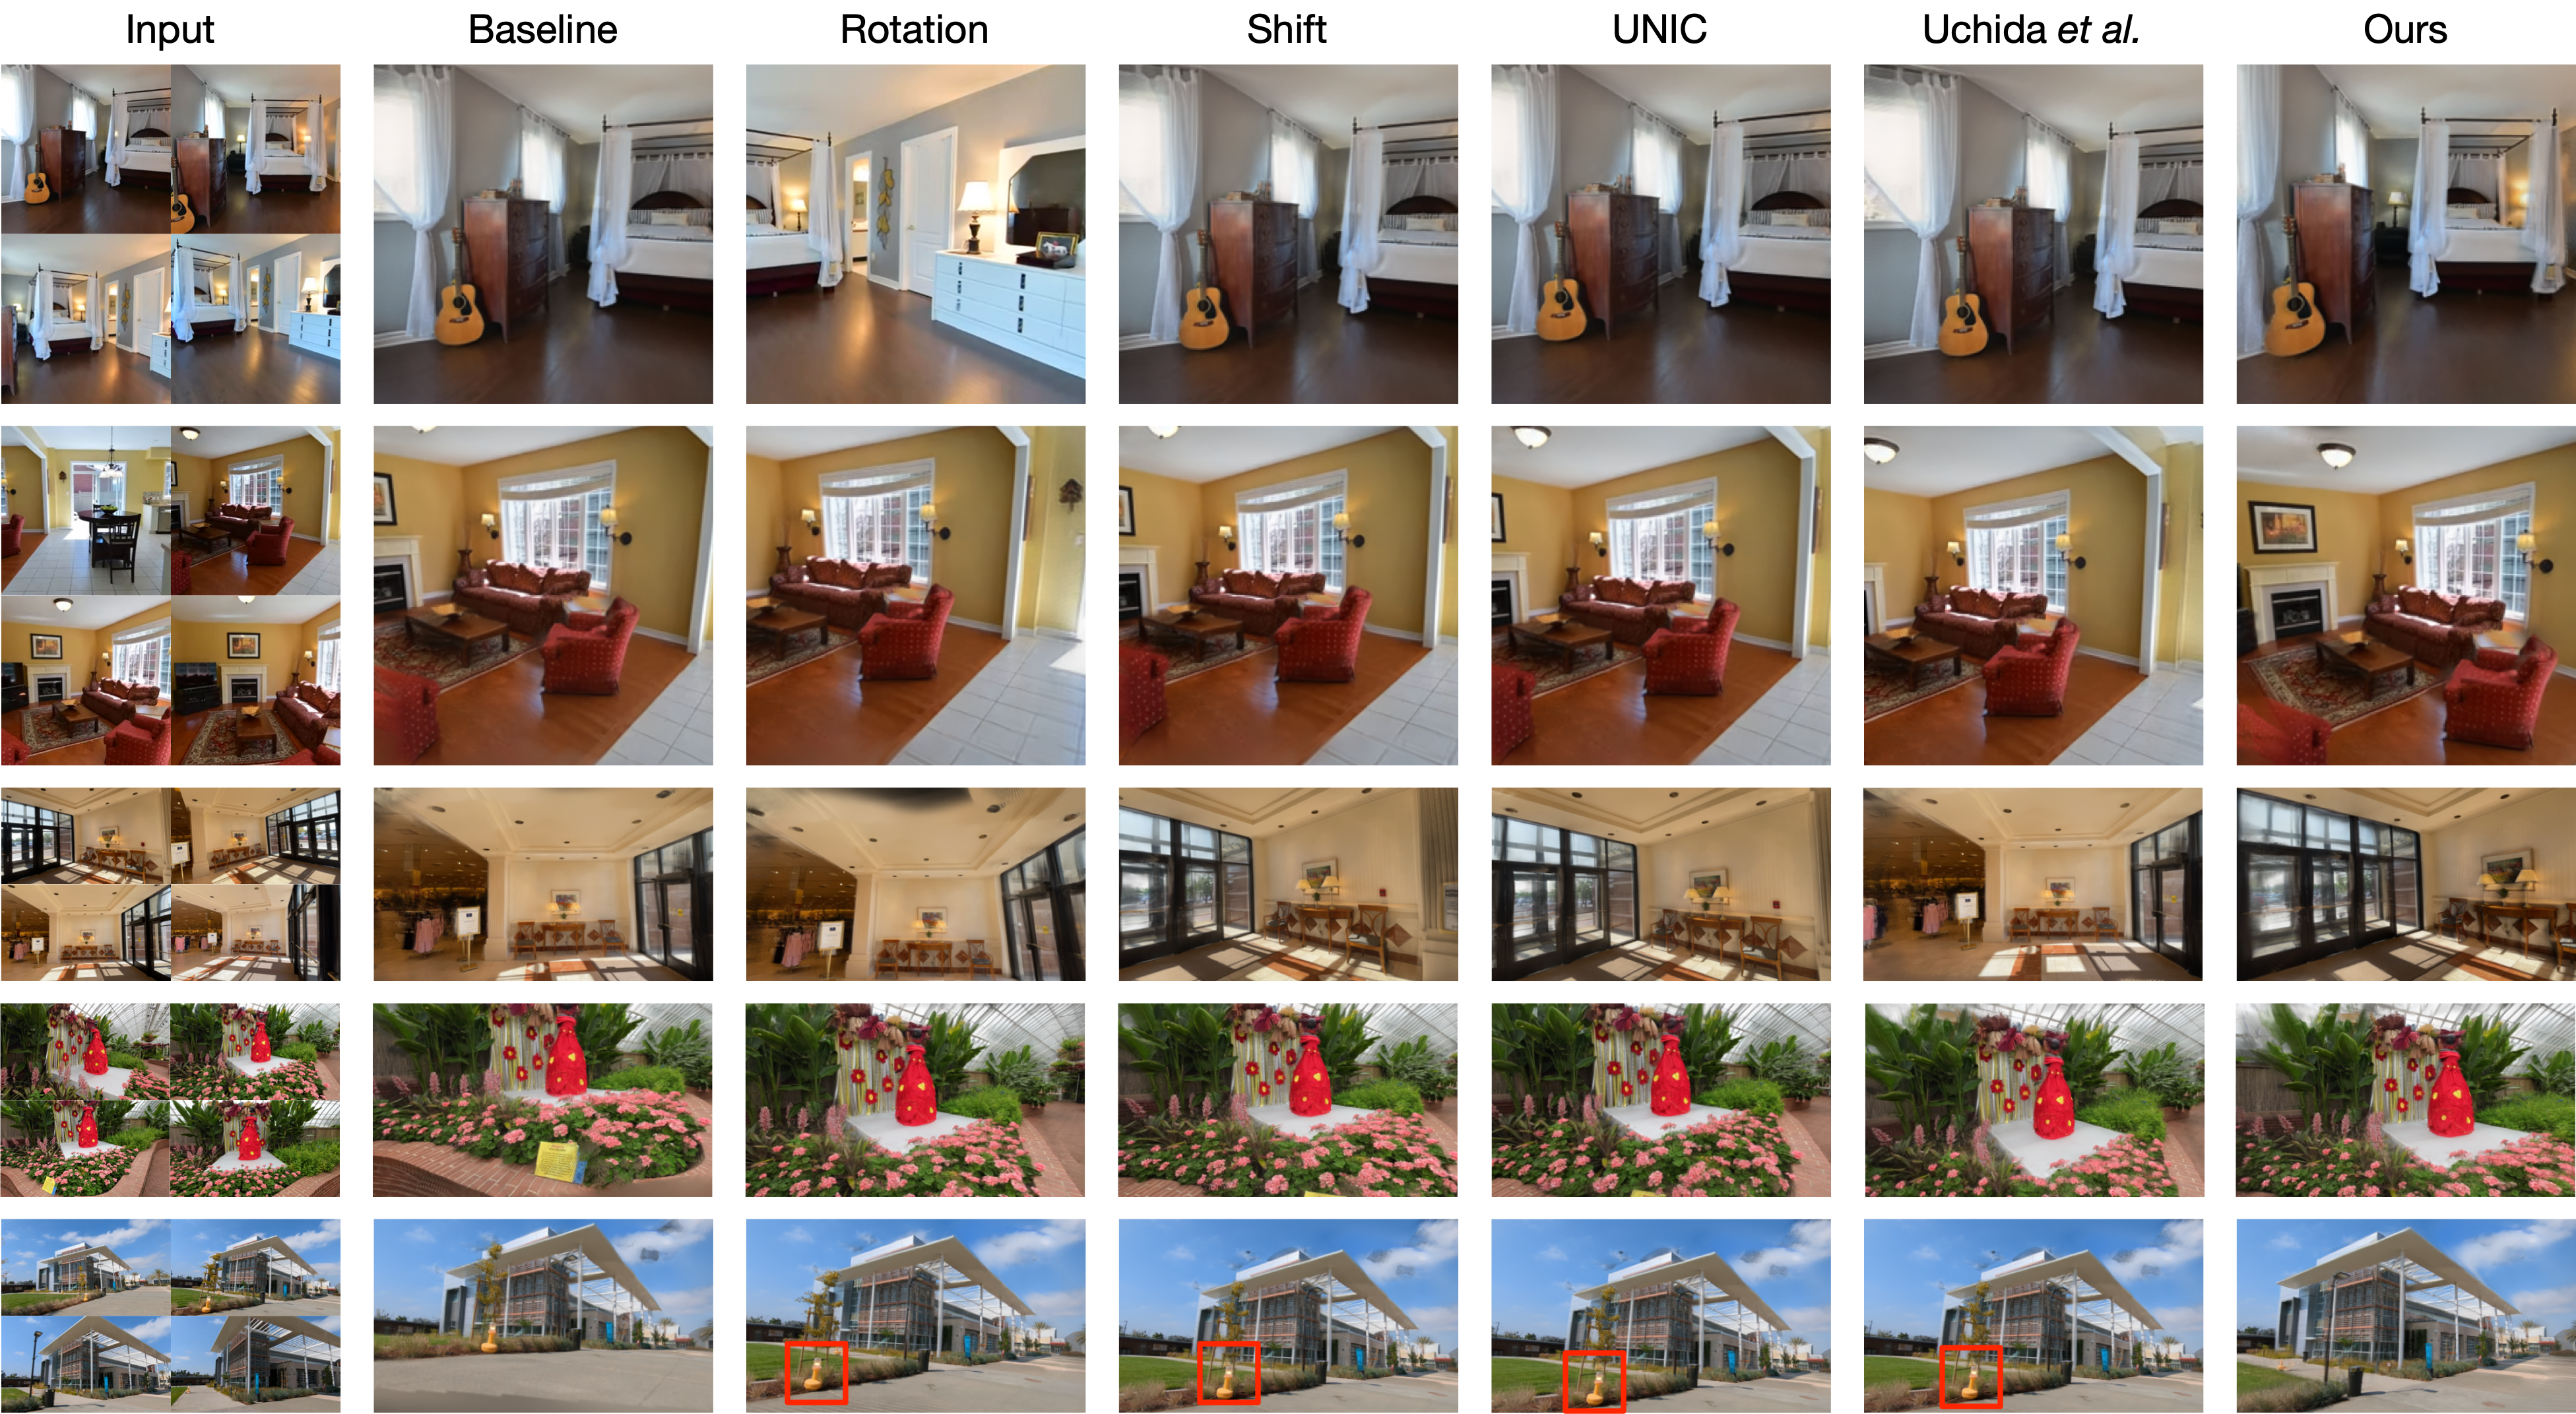
\includegraphics[width=\linewidth]{figs/avs.png}
    \caption{Aesthetic viewpoint suggestion examples with 4 input views in RE10k (\textit{top 2 rows}) and DL3DV (\textit{bottom 3 rows}). Red boxes in the last row show that single-view methods fail to remove distracting objects due to limited adjustment range. Zoom in for more details.}
    \label{fig:avs}
\end{figure*}

\subsection{Aesthetic Viewpoint Suggestion}
To evaluate our method on aesthetic viewpoint suggestion given sparse input views, we vary the number of input views between $[2,4,6]$ and assess the aesthetic quality of the suggested viewpoints. 

Since no existing benchmarks account for viewpoint-dependent aesthetics, we adopt the test splits of RE10k and DL3DV to provide input views and use two aesthetic models (VEN~\cite{wei2018good} and SAMPNet~\cite{sampnet}) to quantify framing and composition quality. Because the suggested views may not have corresponding ground-truth images, we reconstruct the scenes with dense inputs to obtain pseudo ground-truths for evaluation only, ensuring a fair and artifact-mitigated comparison without affecting the viewpoint suggestion process itself. As no prior work operates in this sparse-view setting, we compare against the baseline and single-view methods adapted to our evaluation protocol as detailed below.

\noindent\textbf{Comparison Approaches.} We first compare our method with the direct RGB-scoring baseline, which shares the same search pipeline as ours. To adapt single-view adjustment methods~\cite{li2025towards,su2021camera,uchida20253d,liu2023beyond,yao2025photography,sheng2024view} comparable in our setting, we treat each sparse input view as an anchor, around which we obtain a candidate based on their suggestions. This yields $N$ suggestions for the $N$ input anchors per scene, where we take the best as the final output. 
Among single-view methods, only UNIC~\cite{liu2023beyond} and Uchida \etal~\cite{uchida20253d} are publicly available. 
For fair comparison, we adapt both by fixing their crop sizes as input resolution and map their outpainted suggestions to corresponding real viewpoints. See Supplementary Material for additional details.
% UNIC predicts crops with varying sizes in an extrapolated image plane rather than real camera motions. For fair comparison, we fix its crop size as input resolution and map the crop-center shifts to in-plane camera translations, thereby obtaining corresponding real viewpoints. Similarly, Uchida \etal~\cite{uchida20253d} optimize aesthetics in outpainted 3D scenes; we transform their suggestions to equivalent real viewpoints for evaluation. 
For other methods that predict minor \textit{in-plane shift}~\cite{su2021camera,sheng2024view} or \textit{rotation}~\cite{li2025towards} around the anchor viewpoint, we approximate their behavior by exhaustively sampling and scoring nearby views with the aesthetic model. Yao \etal\cite{yao2025photography} cannot be compared as their video generation model is not available. 3D-exploration methods are not comparable as they need dense captures of the scene.

\noindent\textbf{Quantitative Results.} \Cref{tab:avs} reports the aesthetic viewpoint suggestion results.  
Our method consistently recommends views with higher aesthetic scores than all comparison approaches in different metrics.
It also maintains superior performance across different input numbers, showing robustness under varying observation sparsity. 
Even with only two views, our model produces significantly better suggestions, showing its strong ability to reason about the underlying 3D scene aesthetics from minimal observations.
As the number of input views increases, the suggested viewpoints achieve progressively higher scores, indicating that our model effectively exploits broader scene coverage to discover more aesthetically optimal perspectives.
With more input views, the performance gap over single-view-based methods (\eg \textit{rotation}) narrows, likely because they can also explore sufficient viewpoint variations within their local neighborhoods. However, note that \textit{inplane-shift} and \textit{rotation} serve as an \textit{upper bound} for approximating single-view methods in our setting, as we directly maximize target scores rather than relying on learned guidance.
%Moreover, in practice, single-view methods require multiple physical iterative evaluations around each anchor view. In contrast, our method needs only a single capture per viewpoint, offering a more practical solution.



\noindent\textbf{Qualitative Comparisons.} \Cref{fig:avs} presents qualitative examples of the suggested viewpoints.  
Our framework identifies visually balanced and well-composed views that align with human aesthetic preferences. In contrast, single-view adjustment methods are restricted to small neighborhood around the anchor views and often fail to capture optimal perspectives. For example, they may break the structural continuity of objects (\eg bed frames in the first row) or struggle to remove distracting objects (\eg marked by red boxes in the last row) from the view while our method can freely place the camera to enhance composition.

\begin{figure}[t]
\centering
    
\includegraphics[width=\linewidth]{figs/vis.pdf}
    \caption{Visualization of sampled viewpoints colored by aesthetic score, with representative renderings shown alongside.}
    \label{fig:vis}
\end{figure}


\noindent\textbf{3D Visualization of Viewpoint Suggestions.} Finally, we visualize the viewpoint sampling strategy in~\cref{fig:vis}. Candidate viewpoints are sampled along and around the trajectory of input views, with colors indicating the predicted aesthetic scores. The results reveal how aesthetic quality varies across 3D space, and the corresponding renderings confirm strong alignment with human perceptual preferences.

\begin{table}[t]
\small
  \centering
  \begin{tabular}{l| c c}
    \toprule
    \multirow{2}{*}{Methods}  & RE10k~\cite{re10k} & DL3DV~\cite{dl3dv} \\
      & $\Delta$VEN$\uparrow$ & $\Delta$VEN$\uparrow$ \\
    \midrule
    Baseline & 0.20 & 0.18  \\
    \textbf{Ours} & \textbf{0.46} & \textbf{0.43} \\
    \bottomrule
  \end{tabular}
  \caption{Aesthetic score improvement with gradient ascent.}
  \label{tab:grad}
\end{table}


\subsection{Aesthetic Field Gradient Optimization Analysis}
\label{sec:grad}
We analyze the learned aesthetic field through the lens of gradient-based optimization, and show that the distilled field enables stable and effective gradient ascent compared with the RGB-scoring baseline. We randomly select starting viewpoints and perform gradient ascent on both methods.
For each scene in the test split, both approaches receive the same sparse input views, and the same random novel view is chosen as the initial camera pose for both.  
We run optimization for $25$ steps and report the average score improvement $\Delta$VEN in \cref{tab:grad}.  
Our method achieves consistent score increases in different datasets, confirming that the learned aesthetic field provides a well-behaved optimization landscape.  
In contrast, the RGB-scoring baseline suffers from unstable updates that often degrade the results.
\Cref{fig:grad} further illustrate this behavior. Our method converges toward balanced and aesthetically pleasing viewpoints, while RGB-based refinement fails to update reliably toward better views. See Supplementary Material for more examples.

\begin{figure}[t]
\centering
    \includegraphics[width=\linewidth]{figs/grad_3.pdf}
    \caption{Gradient ascent results. Zoom in for a closer look.}
    \label{fig:grad}
\end{figure}


\subsection{Ablations}
We conduct ablation studies to validate key architectural and configuration choices in our framework.

\noindent\textbf{View-conditioning.} We first examine the role of view-conditioning in aesthetic prediction for novel viewpoints. \cref{tab:ablate_view} shows that view-conditioning significantly improves aesthetic prediction accuracy at unseen views. This confirms that explicitly modeling viewpoint dependence is crucial for capturing aesthetic cues across diverse perspectives.

\begin{table}[t]
\small
  \centering
  \begin{tabular}{l| c c | c c}
    \toprule
    \multirow{2}{*}{Methods}  & \multicolumn{2}{c|}{RE10k~\cite{re10k}} & \multicolumn{2}{c}{DL3DV~\cite{dl3dv}} \\
      & PLCC & SRCC & PLCC & SRCC \\
    \midrule
    w/o. view-cond. & 0.732 & 0.695 & 0.658 & 0.625  \\
    \textbf{w. view-cond.} & \textbf{0.796} & \textbf{0.758} & \textbf{0.700} & \textbf{0.668} \\
    \bottomrule
  \end{tabular}
  \caption{Ablation of view-conditioning on novel view aesthetic prediction with 4 input views.}
  \label{tab:ablate_view}
\end{table}

\noindent\textbf{Search Configurations.} We analyze the number $K$ of candidates returned in coarse sampling and gradient ascent steps in refinement. As shown in \cref{tab:ablate_search}, performance gains saturate around $K=2$ and 25 refinement steps, which are therefore adopted as default in all experiments. Additional ablations are provided in the Supplementary Material.
% We next analyze the search-stage configurations, including the region-based candidate selection and gradient ascent steps. Specifically, we replace the region-based selection with a naive top-1 selection as the candidate in the coarse sampling stage, and compare the resulting performance. As shown in \Cref{tab:ablate_search}, the region-aware selection consistently improves the final suggested viewpoints, demonstrating its effectiveness in mitigating outliers and producing more stable, high-quality recommendations.

% We further vary the number of gradient ascent steps in the refinement stage and measure the average aesthetic score improvement. As shown in \Cref{tab:ablate_step}, the performance gain saturates around 25 steps, which we therefore adopt in all experiments.

% \begin{table}[t]
% \small
%   \centering
%   \begin{tabular}{l | c | c}
%     \toprule
%      \multirow{2}{*}{Methods}  & RE10k~\cite{re10k} & DL3DV~\cite{dl3dv} \\
%      & VEN$\uparrow$ & VEN$\uparrow$ \\
%     \midrule
%     Top-1 & ... & ...  \\
%     \textbf{Region-aware} & \textbf{...} & \textbf{...} \\
%     \bottomrule
%   \end{tabular}
%   \caption{Ablation of candidate selection method in coarse sampling stage.}
%   \label{tab:ablate_search}
% \end{table}

% \begin{table}[t]
% \small
%   \centering
%   \begin{tabular}{l | c | c}
%     \toprule
%      \multirow{2}{*}{\# Steps}  & RE10k~\cite{re10k} & DL3DV~\cite{dl3dv} \\
%      & $\Delta$ VEN$\uparrow$ & $\Delta$ VEN$\uparrow$ \\
%     \midrule
%     15 & 0.21 & 0.15  \\
%     20 & 0.32 & 0.28 \\
%     25 & 0.46 & 0.43 \\
%     30 & 0.49 & 0.45 \\
%     35 & 0.52 & 0.46 \\
%     \bottomrule
%   \end{tabular}
%   \caption{Ablation of gradient update steps in refinement stage.}
%   \label{tab:ablate_step}
% \end{table}

\begin{table}[t]
\small
  \centering
  \begin{tabular}{c | c | c}
    \toprule
    \multirow{2}{*}{\# Candidates} & RE10k~\cite{re10k} & DL3DV~\cite{dl3dv} \\
    & VEN$\uparrow$ & VEN$\uparrow$  \\
    \midrule
    1 & 1.96 & 2.57  \\
    2 &  2.03 & 2.76  \\
    3 &  2.05 & 2.78  \\
    % 4 &  ... & ...  \\
    \midrule
     \# Steps & $\Delta$VEN$\uparrow$ & $\Delta$VEN$\uparrow$ \\
    \midrule
    15 & 0.21 & 0.15 \\
    20 & 0.32 & 0.28 \\
    25 & 0.46 & 0.43 \\
    30 & 0.49 & 0.45 \\
    % 35 & 0.52 & 0.46 \\
    \bottomrule
  \end{tabular}
  \caption{Ablation of candidate numbers and refinement steps.}
  \label{tab:ablate_search}
\end{table}